%================ch2======================================
\chapter{Basic Graph Terminologies}\label{ch2}
\section{Exercises}
    \begin{enumerate}[leftmargin=1.5em]
      \item {
        Show that every regular graph with an odd degree has an even number of vertices.
        
        \begin{description}[leftmargin=0em]
           \item[Answer:] {
                $k$-regular graph of vertices $n$, where $k$ is odd.\\
                Degree sum $= 2m$, where $m$ is number of edges.\\
                $2m = k \times n$\\
                $k$ is odd, $2m$ is even.\\
                $\therefore n$ must be even.
            }
        \end{description}
      }
      \item {
        Construct the complement of $K_{3,3}, W_{5}$, and $C_{5}$.
        
        \begin{description}[leftmargin=0em]
           \item[Answer:] {
                Complement of $K_{3,3}$ Figure \ref{fig:2_2_k}
                \begin{figure}[H]
                    \centering
                    \begin{subfigure}[b]{0.3\textwidth}
                        \centering
                        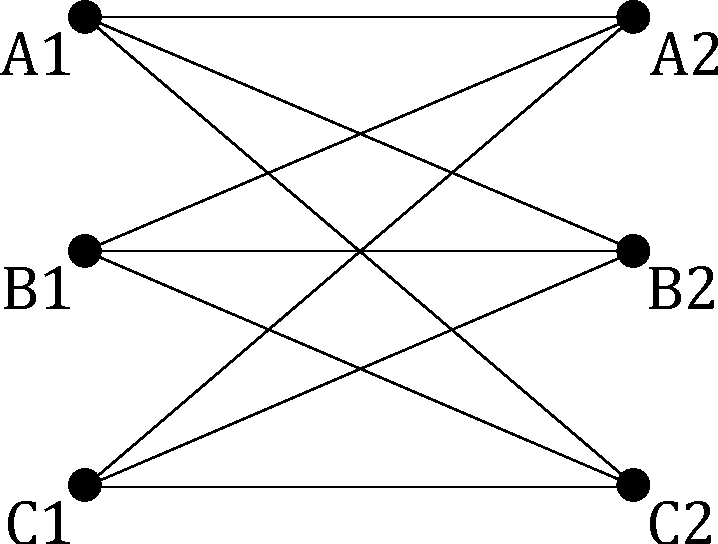
\includegraphics[width = 0.8\textwidth]{2_2_k33.pdf}
                        \caption{$K_{3,3}$}
                        \label{fig:2_2_k33}
                    \end{subfigure}
                    % \hfill
                    \begin{subfigure}[b]{0.4\textwidth}
                        \centering
                        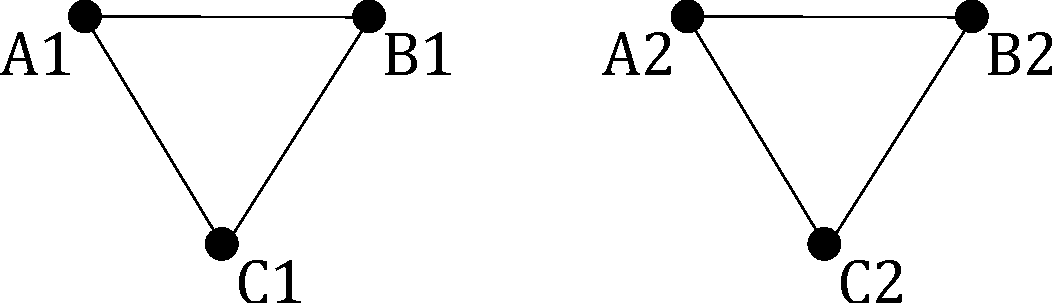
\includegraphics[width = 0.8\textwidth]{2_2_k33_c.pdf}
                        \caption{$\overline{K}_{3,3}$}
                        \label{fig:2_2_k33_c}
                    \end{subfigure}
                    \caption{Complement of $K_{3,3}$}
                    \label{fig:2_2_k}
                \end{figure}
                
                Complement of $W_{5}$ Figure \ref{fig:2_2_w}
                \begin{figure}[H]
                    \centering
                    \begin{subfigure}[b]{0.3\textwidth}
                        \centering
                        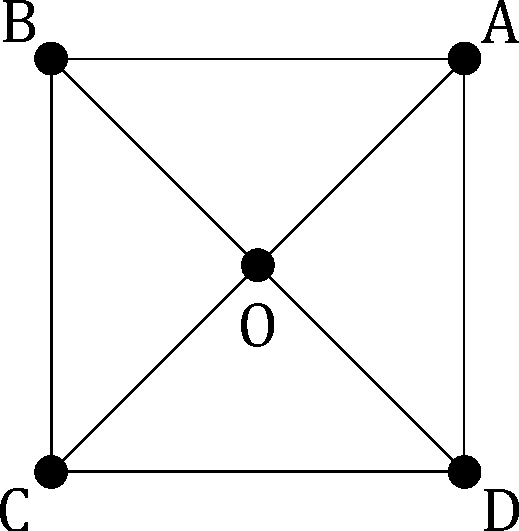
\includegraphics[width = 0.8\textwidth]{2_2_w5.pdf}
                        \caption{$W_{5}$}
                        \label{fig:2_2_w5}
                    \end{subfigure}
                    % \hfill
                    \begin{subfigure}[b]{0.4\textwidth}
                        \centering
                        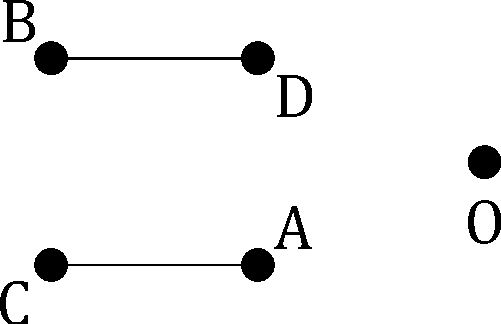
\includegraphics[width = 0.8\textwidth]{2_2_w5_c.pdf}
                        \caption{$\overline{W}_{5}$}
                        \label{fig:2_2_w5_c}
                    \end{subfigure}
                    \caption{Complement of $W_{5}$}
                    \label{fig:2_2_w}
                \end{figure}
                
                Complement of $C_{5}$ Figure \ref{fig:2_2_c}
                \begin{figure}[H]
                    \centering
                    \begin{subfigure}[b]{0.3\textwidth}
                        \centering
                        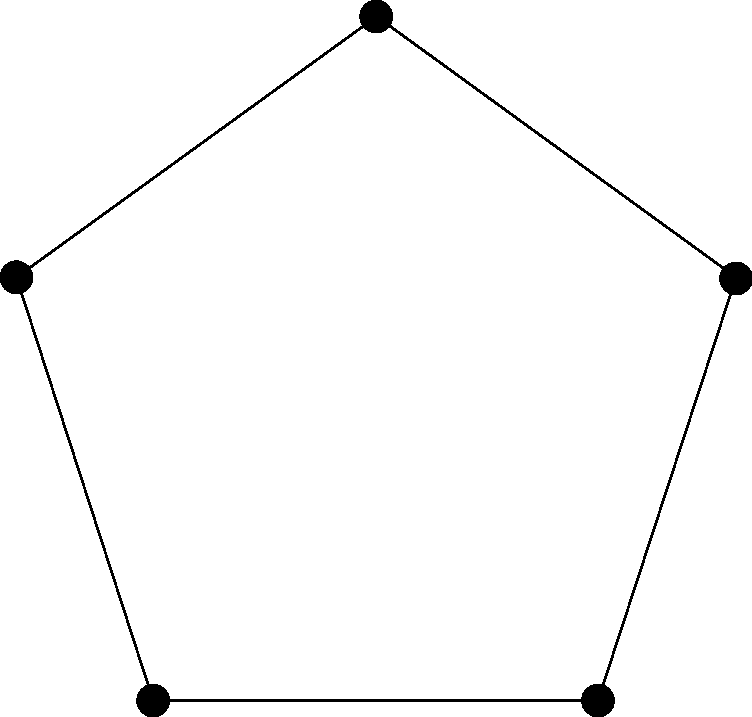
\includegraphics[width = 0.8\textwidth]{2_2_c5.pdf}
                        \caption{$C_{5}$}
                        \label{fig:2_2_c5}
                    \end{subfigure}
                    % \hfill
                    \begin{subfigure}[b]{0.3\textwidth}
                        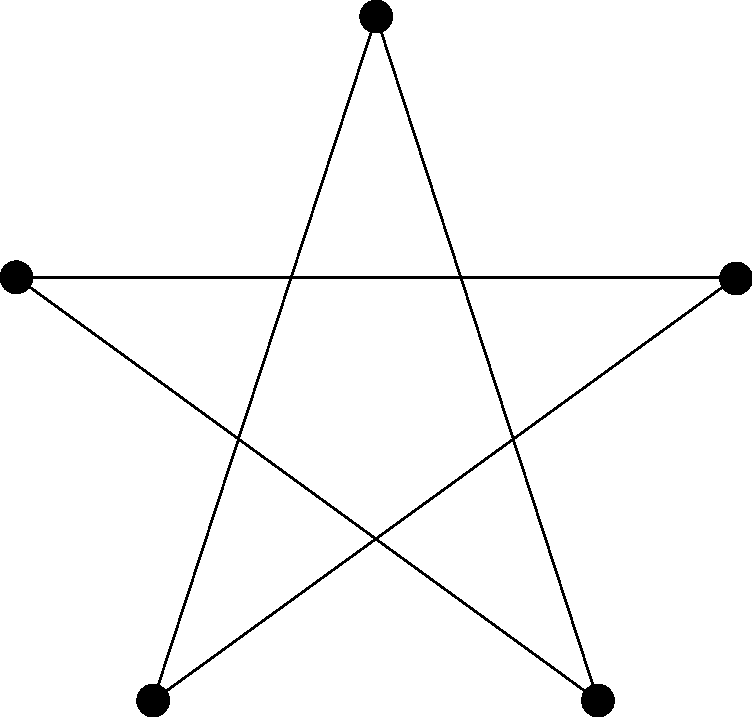
\includegraphics[width = 0.8\textwidth]{2_2_c5_c.pdf}
                        \caption{$\overline{C}_{5}$}
                        \label{fig:2_2_c5_c}
                    \end{subfigure}
                    \caption{Complement of $C_{5}$}
                    \label{fig:2_2_c}
                \end{figure}
            }
        \end{description}
      }
      \item {
        Can you construct a disconnected graph $G$ of two or more vertices such that $	\overline{G}$ is also disconnected. Give a proof supporting your answer.
        
        \begin{description}[leftmargin=0em]
           \item[Answer:] {
                No.\\
                Let us prove given a graph $G$ of two or more vertices, either $G$ or $\overline{G}$ is connected. \\
                $G$ is disconnected. We want to show that $\overline{G}$ is connected. \\
                Suppose $v$ and $w$ are vertices. If $(v, w)$ is not an edge in $G$, then it is an edge in $\overline{G}$, and so we have a path from $v$ to $w$ in $\overline{G}$. On the other hand, if $(v, w)$ is an edge in $G$, then this means $v$ and $w$ are in the same component of $G$. Since $G$ is disconnected, we can find a vertex $u$ in a different component, so that neither $(v, u)$ nor $(u, w)$ are edges of $G$. Then $(v, u, w)$ is a path from $v$ to $w$ in $\overline{G}$. \\
                This shows that any two vertices in $\overline{G}$ have a path (in fact a path of length one or two) between them in $\overline{G}$, so $\overline{G}$ is connected. \cite{122188}
                
                Example Figure \ref{fig:2_3_disc_g}:
                \begin{figure}[H]
                    \centering
                    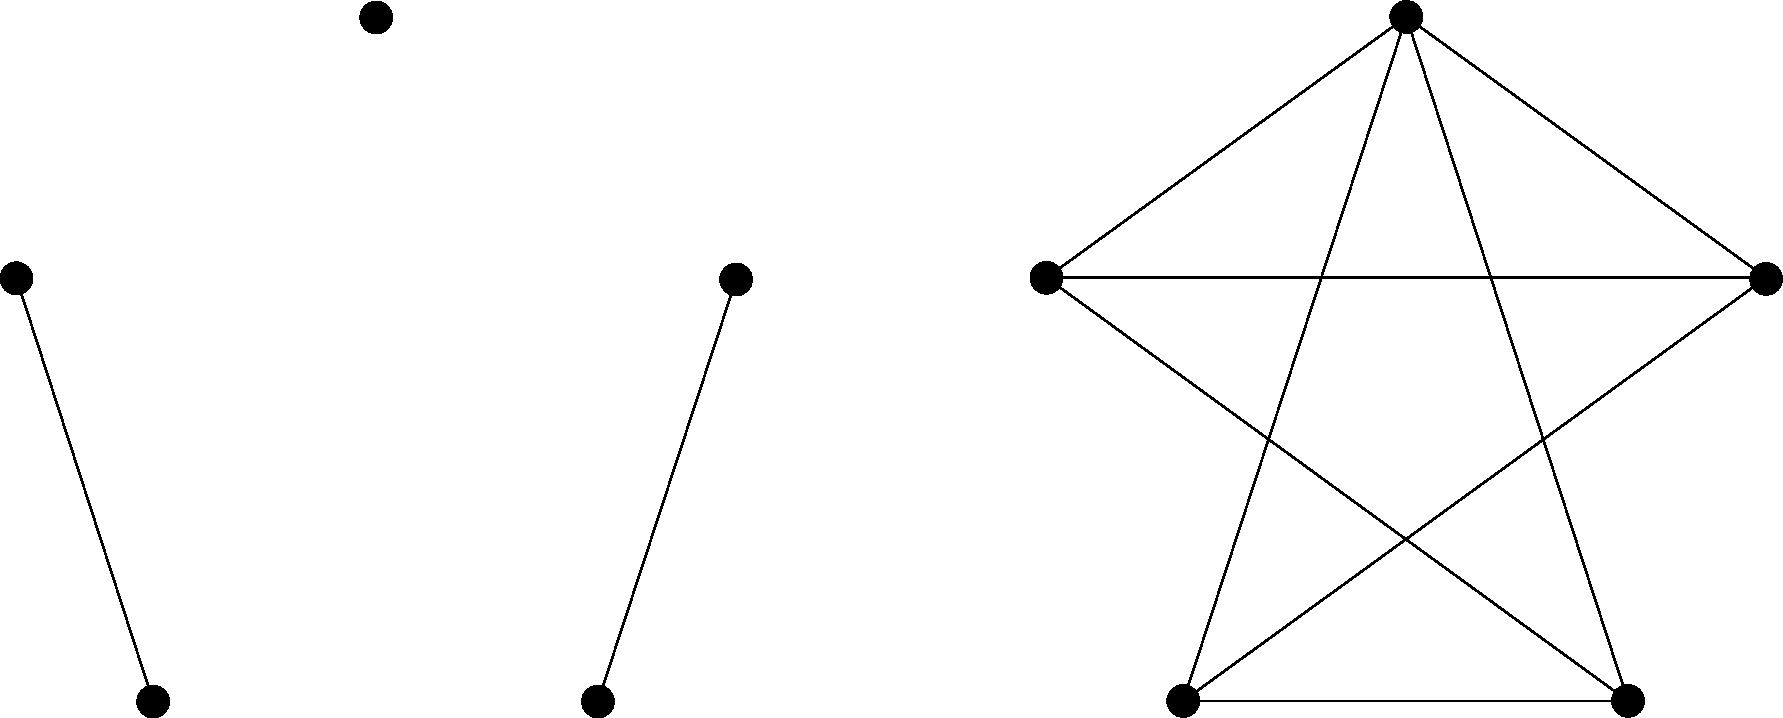
\includegraphics[width = 0.8\textwidth]{2_3_disc_g.pdf}
                    \caption{Complement of disconnected graph is connected example}
                    \label{fig:2_3_disc_g}
                \end{figure}
            }
        \end{description}
      }
      \item {
        Give two examples of self-complementary graphs.
        
        \begin{description}[leftmargin=0em]
           \item[Answer:] {
                Self complementary graphs example: $C_5$, $P_4$ Figure \ref{fig:2_4_self_compl}
                \begin{figure}[H]
                    \centering
                    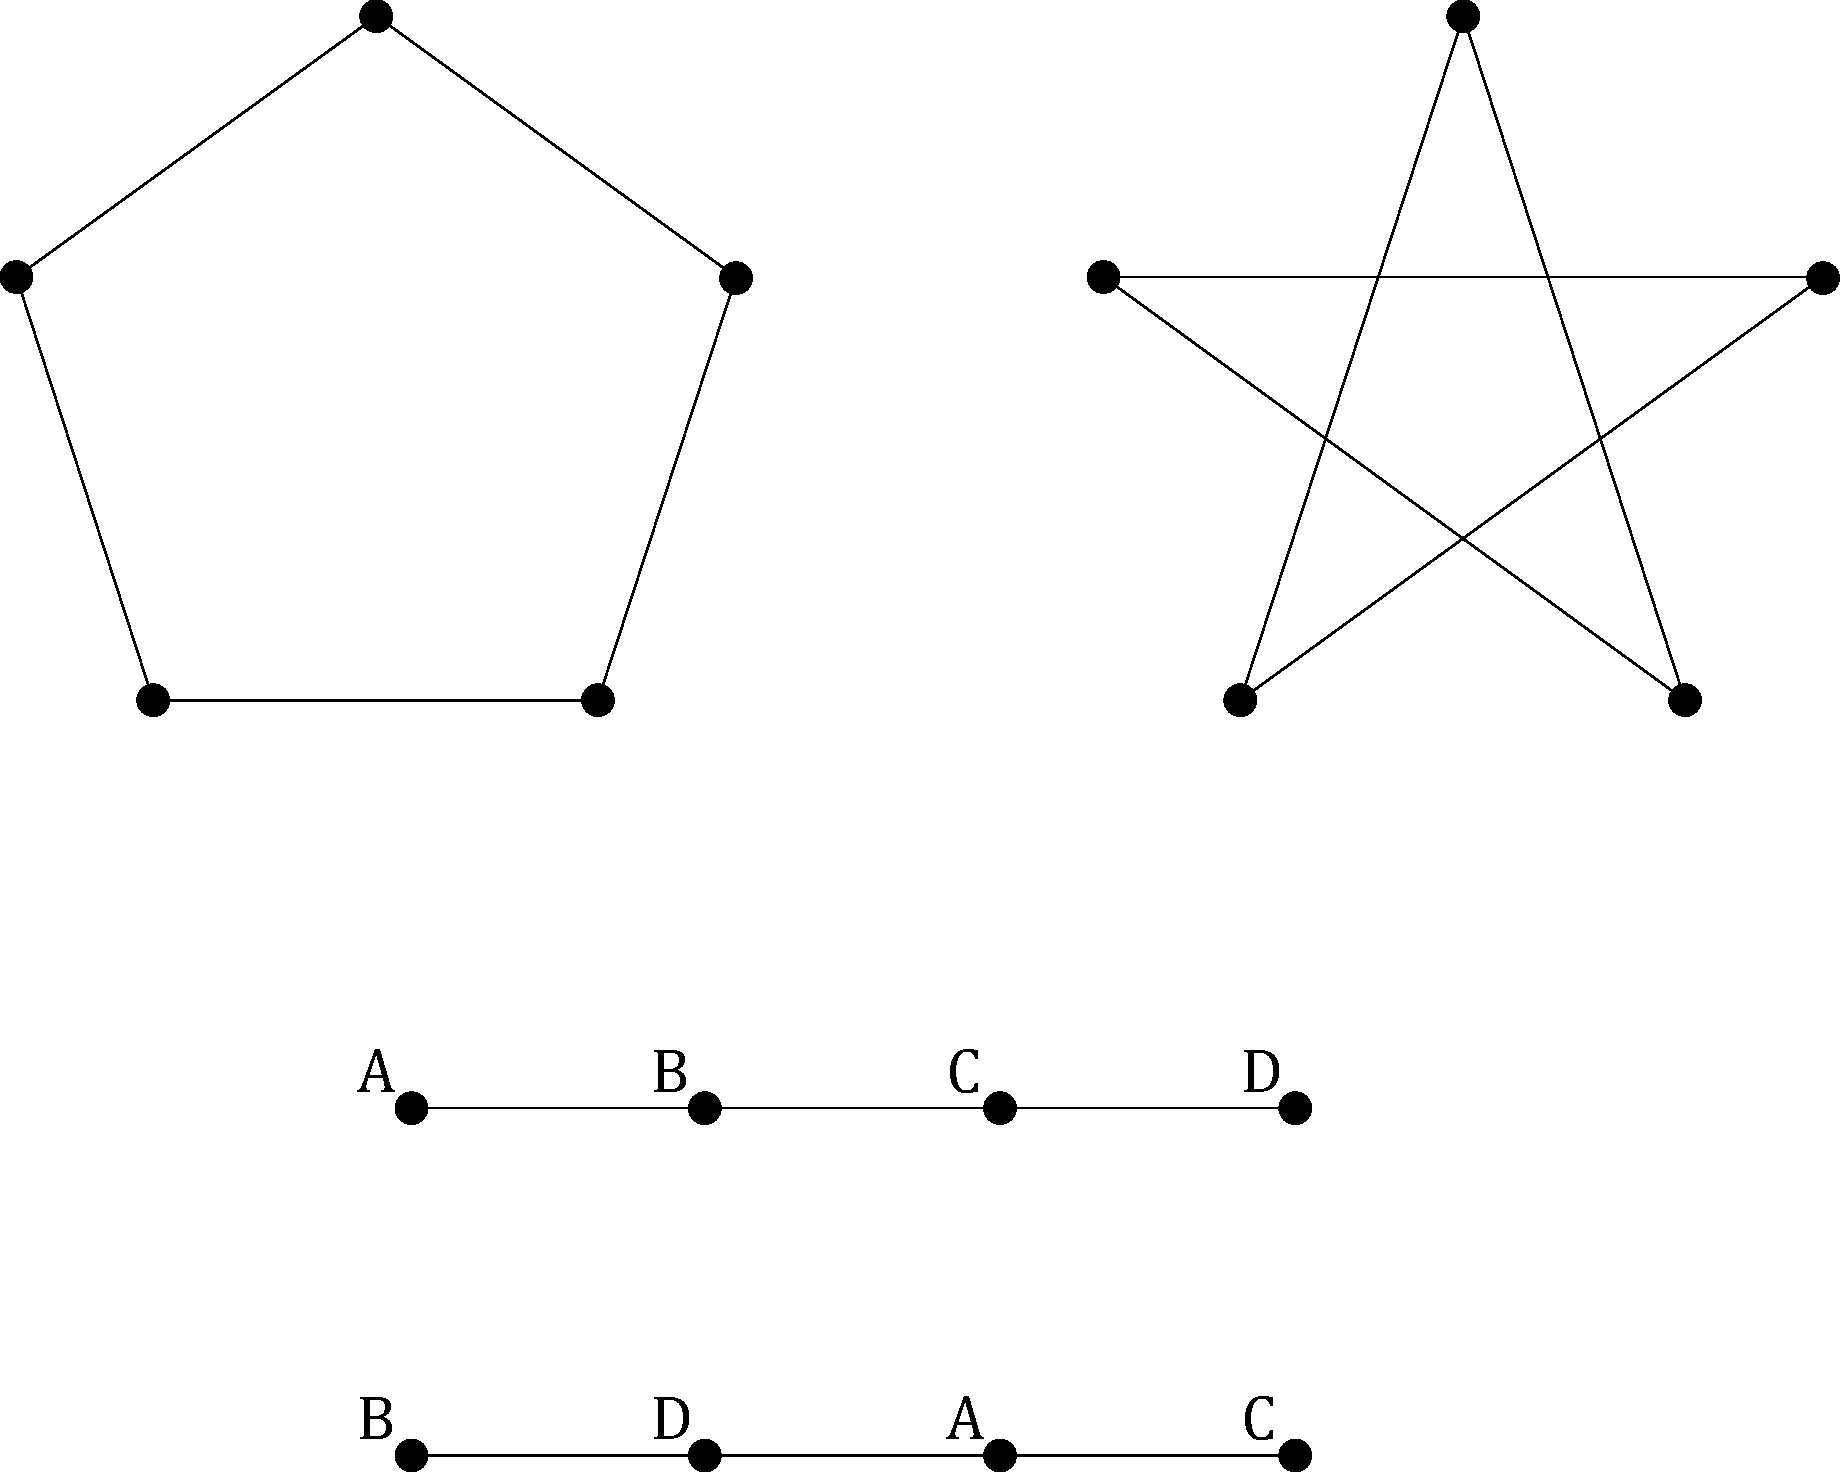
\includegraphics[width = 0.8\textwidth]{2_4_self_compl.pdf}
                    \caption{Self complementary graphs $C_5$, $P_4$}
                    \label{fig:2_4_self_compl}
                \end{figure}
            }
        \end{description}
      }
      \item {
        What is the necessary and sufficient condition for $K_{m,n}$ to be a regular graph?
        
        \begin{description}[leftmargin=0em]
           \item[Answer:] {
                In the complete bipartite graph $K_{m,n}$, the vertices have degree $m$ or degree $n$ (and both of these degrees are reached). Thus, to be regular, a sufficient and necessary condition is $n=m$. \cite{3733224}
            }
        \end{description}
      }
      \item {
        Is there a simple graph of $n$ vertices such that the vertices all have distinct degrees? Give a proof supporting your answer.
        
        \begin{description}[leftmargin=0em]
           \item[Answer:] {
                If $n=1$, yes, trivial. \\
                For $n>1$. Suppose such a graph exists. Each vertex in the graph can have a degree from $0$ to $n-1$ (simple graphs do not forbid a degree-$0$ vertex, \emph{connected} graphs do). Since this range spans $n$ values in total and each vertex degree is different, the degrees are distributed one-per-vertex. In particular, there must exist a vertex with degree $n-1$ and one with degree $0$. \\
                Now the degree-$n-1$ vertex is connected to all other vertices because the graph is simple, \emph{including} the degree-$0$ vertex. But the latter is not connected to any vertex, which is a contradiction. Therefore two vertices in the graph must have the same degree.
                \cite{2690153} \cite{202585439}
            }
        \end{description}
      }
      \item {
        Draw the graph $G = (V, E)$ with vertex set $V = \{a, b, c, d, e, f, g, h\}$ and edge set $\{(a, b), (a, e), (b, c), (b, d), (c, d), (c, g), (d, e)(e, f ), ( f, g), ( f, h), (g, h)\}$. Draw $G - (d, e)$. Draw the subgraph of $G$ induced by $\{c, d, e, f\}$. Contract the edge $(d, e)$ from $G$.
        
        \begin{description}[leftmargin=0em]
           \item[Answer:] {
                Graph drawings Figure \ref{fig:2_7}
                \begin{figure}[ht]
                    \centering
                    \begin{subfigure}[b]{0.4\textwidth}
                        \centering
                        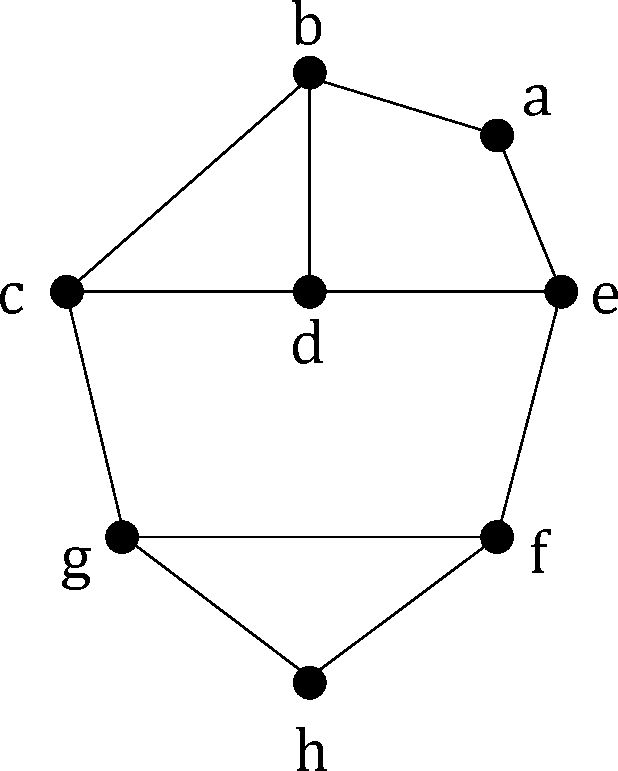
\includegraphics[width = 0.8\textwidth]{2_7_G.pdf}
                        \caption{$G$}
                        \label{fig:2_7_G}
                    \end{subfigure}
                    % \hfill
                    \begin{subfigure}[b]{0.4\textwidth}
                        \centering
                        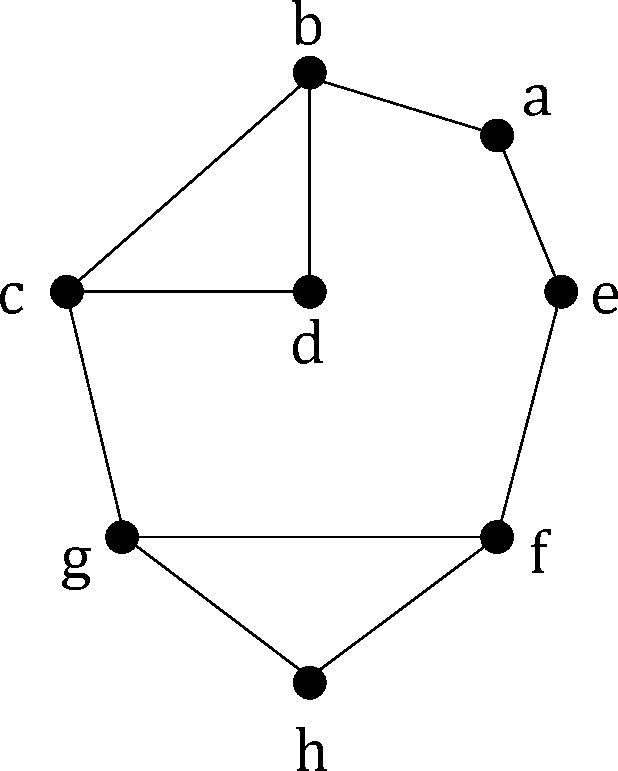
\includegraphics[width = 0.8\textwidth]{2_7_G-d_e.pdf}
                        \caption{$G-(d,e)$}
                        \label{fig:2_7_G-d_e}
                    \end{subfigure}
                    % \hfill
                    \begin{subfigure}[b]{0.4\textwidth}
                        \centering
                        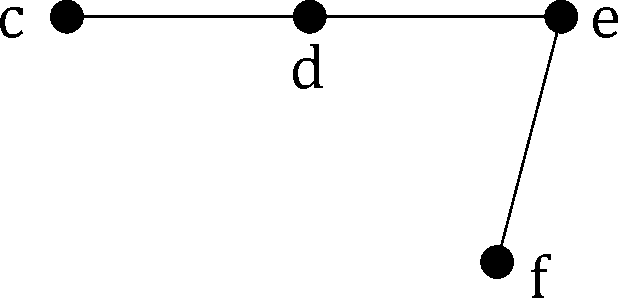
\includegraphics[width = 0.8\textwidth]{2_7_c_d_e_f.pdf}
                        \caption{$G$ induced by $\{c, d, e, f\}$}
                        \label{fig:2_7_c_d_e_f}
                    \end{subfigure}
                    % \hfill
                    \begin{subfigure}[b]{0.4\textwidth}
                        \centering
                        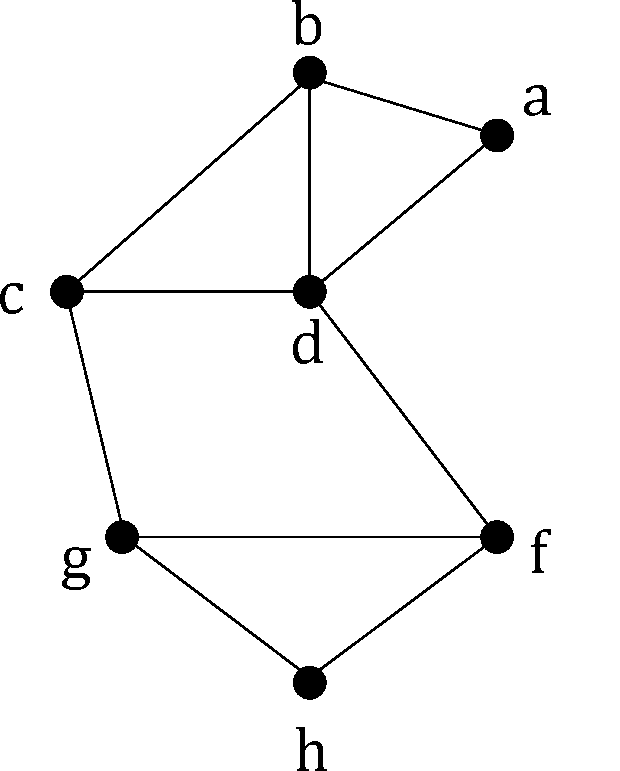
\includegraphics[width = 0.8\textwidth]{2_7_G-d_e_contr.pdf}
                        \caption{$(d, e)$ edge contracted from $G$}
                        \label{fig:2_7_G-d_e_contr}
                    \end{subfigure}
                    
                    \caption{Graph drawings}
                    \label{fig:2_7}
                \end{figure}
            }
        \end{description}
      }
      \item {
        Show that two graphs are isomorphic if and only if their complements are isomorphic.
        
        \begin{description}[leftmargin=0em]
           \item[Answer:] {
                Let graph $G$ be isomorphic to $H$, and let $\overline G$, $\overline H$ denote their complements. \\
                Since $G$ is isomorphic to $H$, then there exists a bijection $f: V(G) \to V(H)$, such that $(u, v) \in E(G)$ if and only if $(f(u), f(v)) \in E(H)$. \\
                Equivalently, there exists a bijection $f: V(G) \to V(H)$, such that $(u, v) \notin E(G)$ if and only if $(f(u), f(v)) \notin E(H)$. \\
                Since the vertex set of $G$ and $\overline G$ are the same, therefore $f$ is a bijection from $V(\overline G)$ to $V(\overline H)$. Then suppose $(u, v) \notin E(G)$, by definition of a complement, $(u, v) \in E(\overline G)$. Likewise, if $(f(u), f(v)) \notin E(H)$, then $(f(u), f(v)) \in E(\overline H)$. \\
                Hence $\overline G$ and $\overline H$ are isomorphic. \cite{2451171}
            }
        \end{description}
      }
    \end{enumerate}
    
% \section{Solutions}
%     \begin{enumerate}[leftmargin=1.5em]
%       \item {
%         % Show that every regular graph with an odd degree has an even number of vertices.
        
%         \begin{description}[leftmargin=0em]
%           \item[Answer:] {
%                 $k$-regular graph of vertices $n$, where $k$ is odd.\\
%                 Degree sum $= 2m$, where $m$ is number of edges.\\
%                 $2m = k \times n$\\
%                 $k$ is odd, $2m$ is even.\\
%                 $\therefore n$ must be even.
%             }
%         \end{description}
%       }
%       \item {
%         % Construct the complement of $K_{3,3}, W_{5}$, and $C_{5}$.
        
%         \begin{description}[leftmargin=0em]
%           \item[Answer:] {
%                 Complement of $K_{3,3}$ Figure \ref{fig:2_2_k}
%                 \begin{figure}[H]
%                     \centering
%                     \begin{subfigure}[b]{0.3\textwidth}
%                         \centering
%                         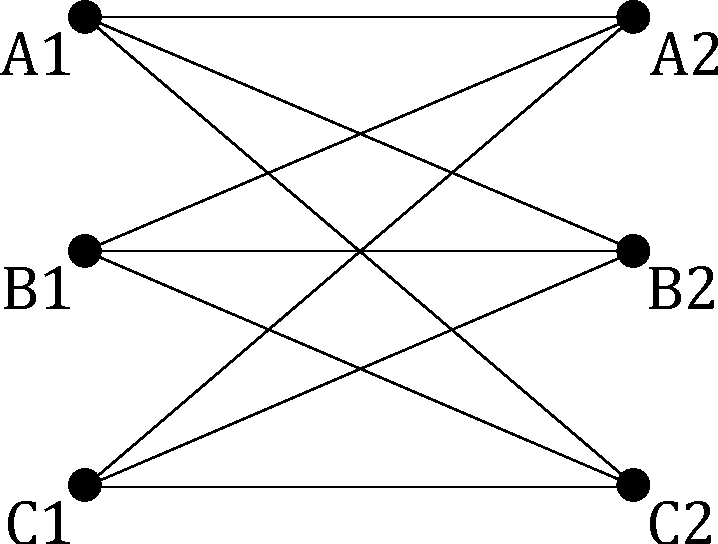
\includegraphics[width = 0.8\textwidth]{2_2_k33.pdf}
%                         \caption{$K_{3,3}$}
%                         \label{fig:2_2_k33}
%                     \end{subfigure}
%                     % \hfill
%                     \begin{subfigure}[b]{0.4\textwidth}
%                         \centering
%                         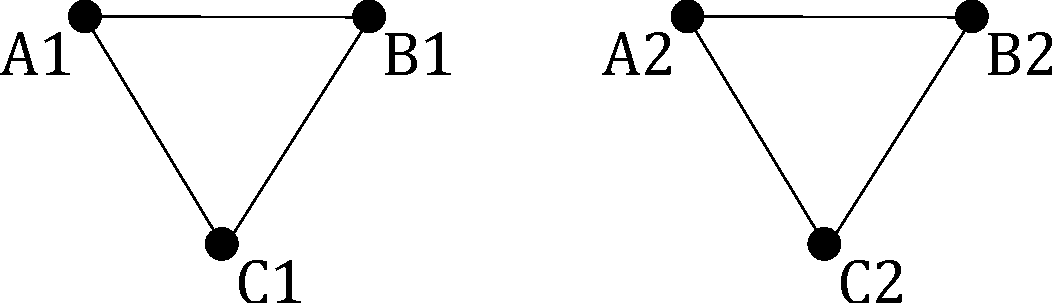
\includegraphics[width = 0.8\textwidth]{2_2_k33_c.pdf}
%                         \caption{$\overline{K}_{3,3}$}
%                         \label{fig:2_2_k33_c}
%                     \end{subfigure}
%                     \caption{Complement of $K_{3,3}$}
%                     \label{fig:2_2_k}
%                 \end{figure}
                
%                 Complement of $W_{5}$ Figure \ref{fig:2_2_w}
%                 \begin{figure}[H]
%                     \centering
%                     \begin{subfigure}[b]{0.3\textwidth}
%                         \centering
%                         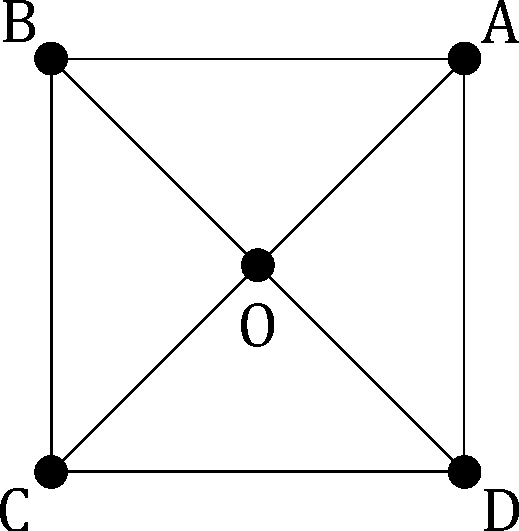
\includegraphics[width = 0.8\textwidth]{2_2_w5.pdf}
%                         \caption{$W_{5}$}
%                         \label{fig:2_2_w5}
%                     \end{subfigure}
%                     % \hfill
%                     \begin{subfigure}[b]{0.4\textwidth}
%                         \centering
%                         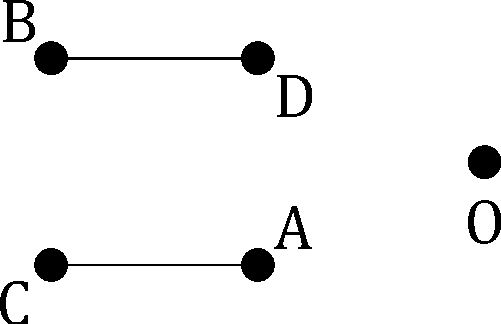
\includegraphics[width = 0.8\textwidth]{2_2_w5_c.pdf}
%                         \caption{$\overline{W}_{5}$}
%                         \label{fig:2_2_w5_c}
%                     \end{subfigure}
%                     \caption{Complement of $W_{5}$}
%                     \label{fig:2_2_w}
%                 \end{figure}
                
%                 Complement of $C_{5}$ Figure \ref{fig:2_2_c}
%                 \begin{figure}[H]
%                     \centering
%                     \begin{subfigure}[b]{0.3\textwidth}
%                         \centering
%                         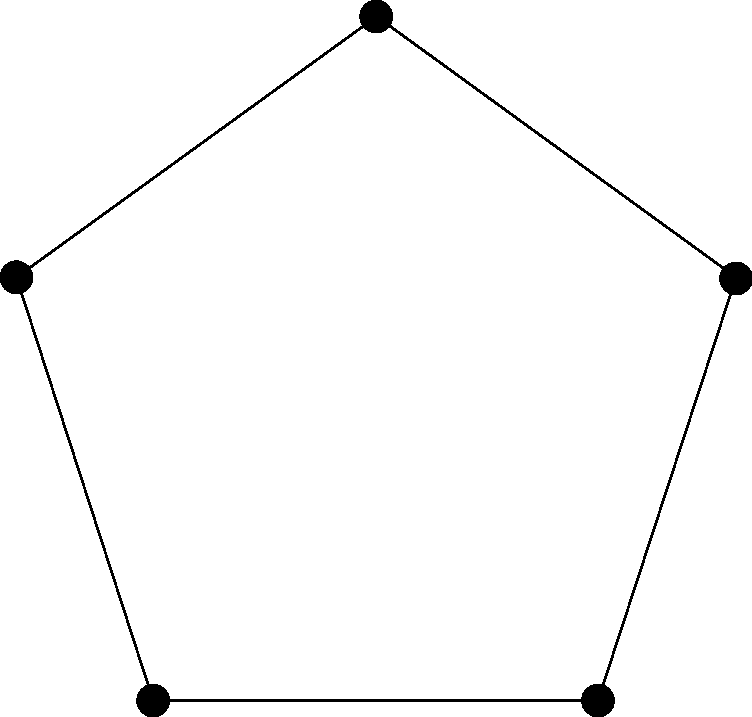
\includegraphics[width = 0.8\textwidth]{2_2_c5.pdf}
%                         \caption{$C_{5}$}
%                         \label{fig:2_2_c5}
%                     \end{subfigure}
%                     % \hfill
%                     \begin{subfigure}[b]{0.3\textwidth}
%                         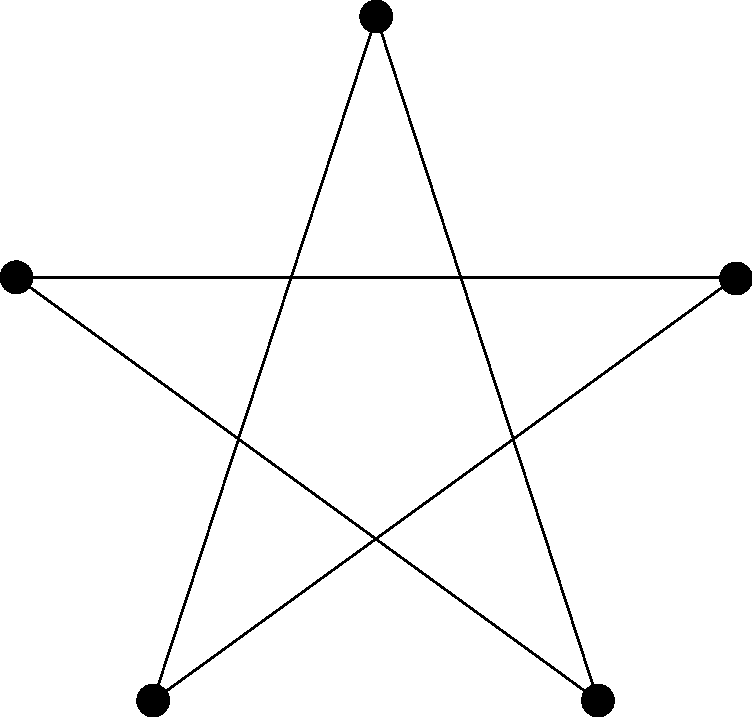
\includegraphics[width = 0.8\textwidth]{2_2_c5_c.pdf}
%                         \caption{$\overline{C}_{5}$}
%                         \label{fig:2_2_c5_c}
%                     \end{subfigure}
%                     \caption{Complement of $C_{5}$}
%                     \label{fig:2_2_c}
%                 \end{figure}
%             }
%         \end{description}
%       }
%       \item {
%         % Can you construct a disconnected graph $G$ of two or more vertices such that $	\overline{G}$ is also disconnected. Give a proof supporting your answer.
        
%         \begin{description}[leftmargin=0em]
%           \item[Answer:] {
%                 No.\\
%                 Let us prove given a graph $G$ of two or more vertices, either $G$ or $\overline{G}$ is connected. \\
%                 $G$ is disconnected. We want to show that $\overline{G}$ is connected. \\
%                 Suppose $v$ and $w$ are vertices. If $(v, w)$ is not an edge in $G$, then it is an edge in $\overline{G}$, and so we have a path from $v$ to $w$ in $\overline{G}$. On the other hand, if $(v, w)$ is an edge in $G$, then this means $v$ and $w$ are in the same component of $G$. Since $G$ is disconnected, we can find a vertex $u$ in a different component, so that neither $(v, u)$ nor $(u, w)$ are edges of $G$. Then $(v, u, w)$ is a path from $v$ to $w$ in $\overline{G}$. \\
%                 This shows that any two vertices in $\overline{G}$ have a path (in fact a path of length one or two) between them in $\overline{G}$, so $\overline{G}$ is connected. \cite{122188}
                
%                 Example Figure \ref{fig:2_3_disc_g}:
%                 \begin{figure}[H]
%                     \centering
%                     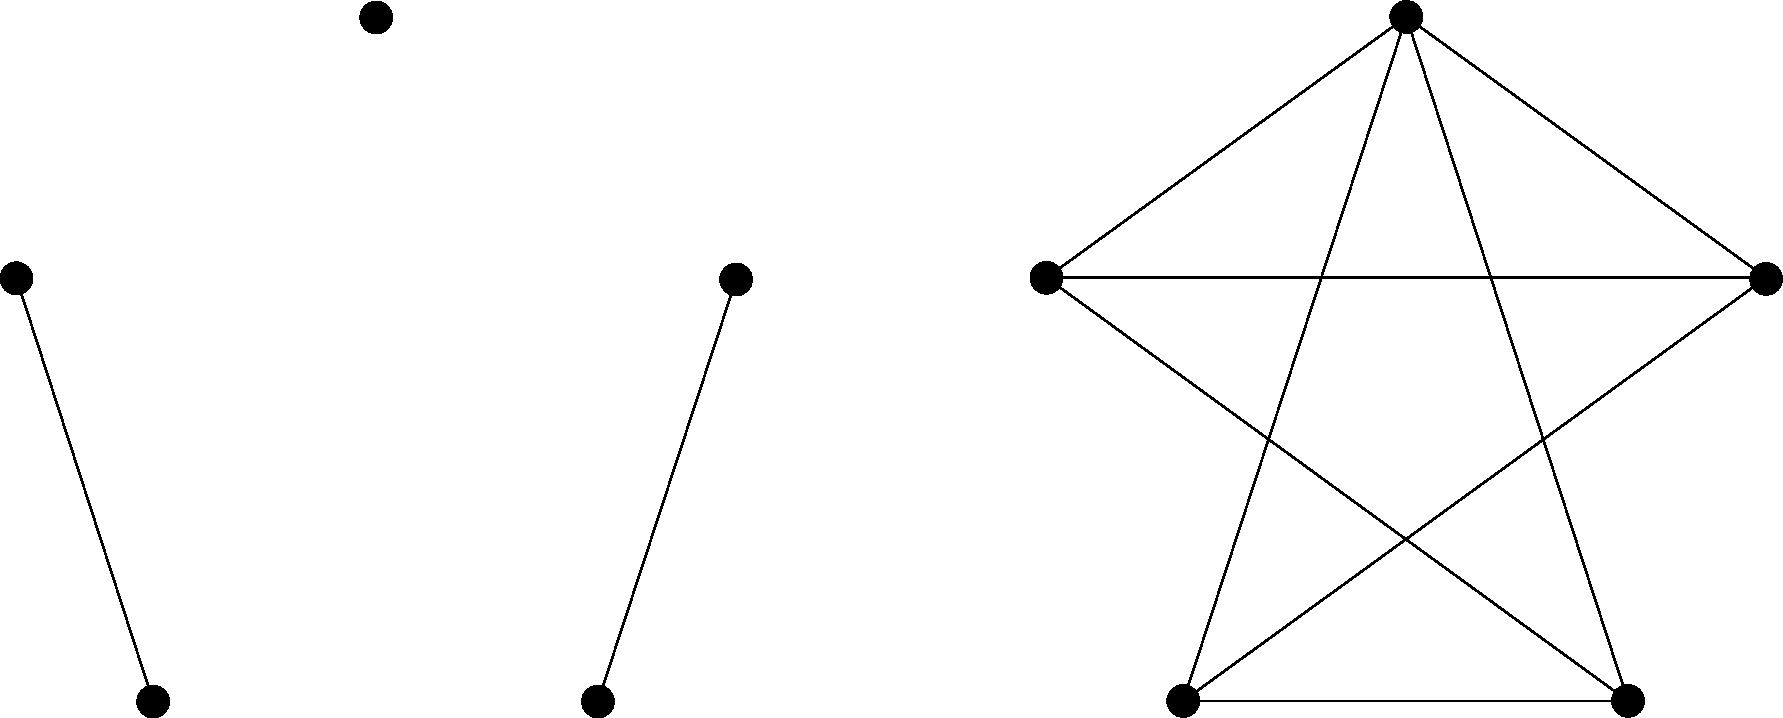
\includegraphics[width = 0.8\textwidth]{2_3_disc_g.pdf}
%                     \caption{Complement of disconnected graph is connected example}
%                     \label{fig:2_3_disc_g}
%                 \end{figure}
%             }
%         \end{description}
%       }
%       \item {
%         % Give two examples of self-complementary graphs.
        
%         \begin{description}[leftmargin=0em]
%           \item[Answer:] {
%                 Self complementary graphs example: $C_5$, $P_4$ Figure \ref{fig:2_4_self_compl}
%                 \begin{figure}[H]
%                     \centering
%                     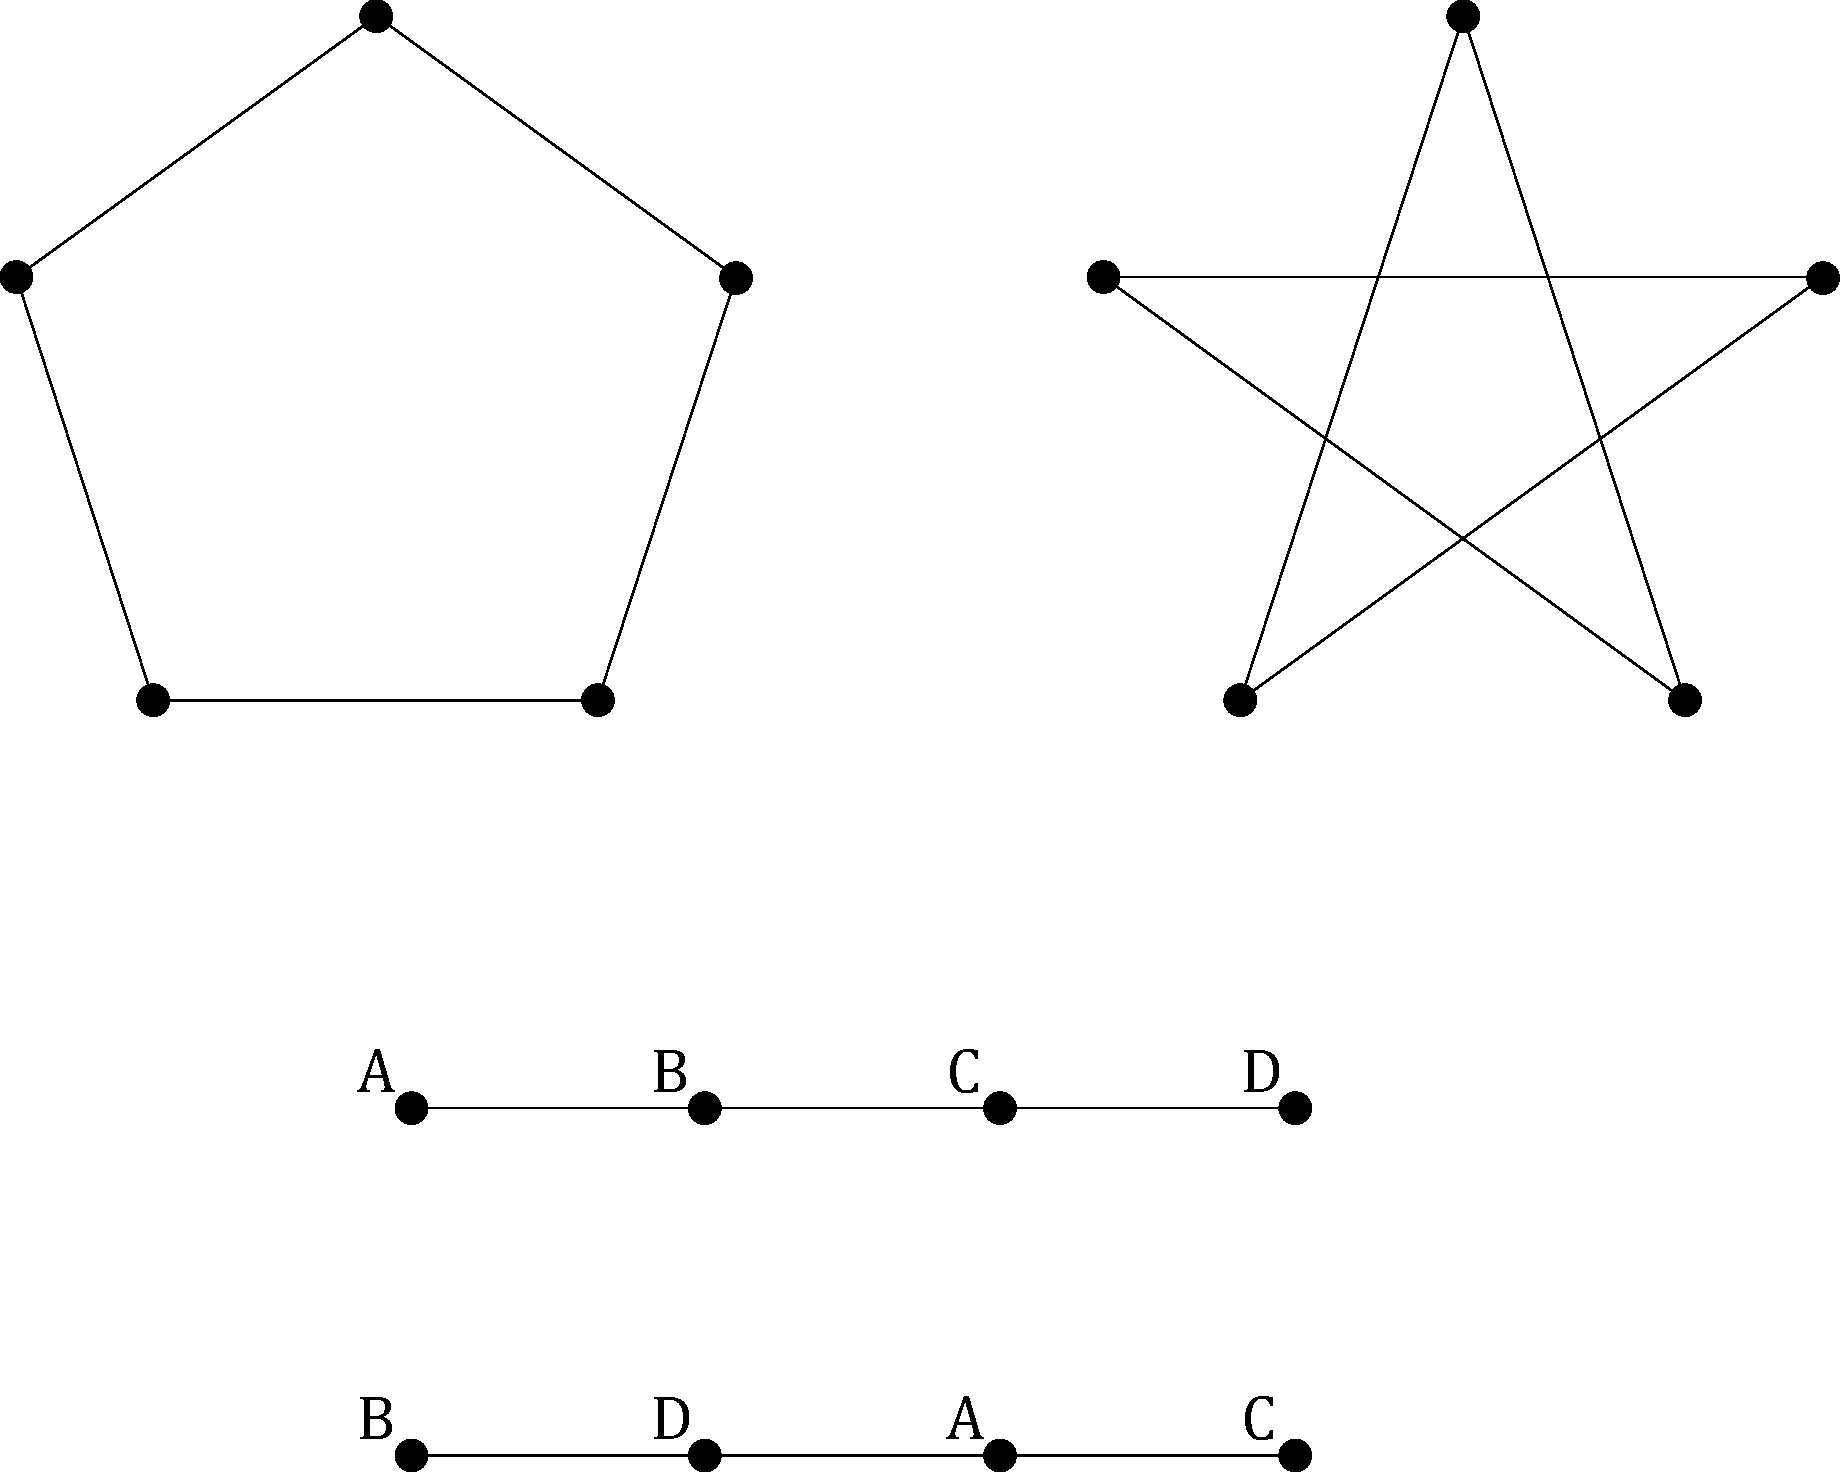
\includegraphics[width = 0.8\textwidth]{2_4_self_compl.pdf}
%                     \caption{Self complementary graphs $C_5$, $P_4$}
%                     \label{fig:2_4_self_compl}
%                 \end{figure}
%             }
%         \end{description}
%       }
%       \item {
%         % What is the necessary and sufficient condition for $K_{m,n}$ to be a regular graph?
        
%         \begin{description}[leftmargin=0em]
%           \item[Answer:] {
%                 In the complete bipartite graph $K_{m,n}$, the vertices have degree $m$ or degree $n$ (and both of these degrees are reached). Thus, to be regular, a sufficient and necessary condition is $n=m$. \cite{3733224}
%             }
%         \end{description}
%       }
%       \item {
%         % Is there a simple graph of $n$ vertices such that the vertices all have distinct degrees? Give a proof supporting your answer.
        
%         \begin{description}[leftmargin=0em]
%           \item[Answer:] {
%                 If $n=1$, yes, trivial. \\
%                 For $n>1$. Suppose such a graph exists. Each vertex in the graph can have a degree from $0$ to $n-1$ (simple graphs do not forbid a degree-$0$ vertex, \emph{connected} graphs do). Since this range spans $n$ values in total and each vertex degree is different, the degrees are distributed one-per-vertex. In particular, there must exist a vertex with degree $n-1$ and one with degree $0$. \\
%                 Now the degree-$n-1$ vertex is connected to all other vertices because the graph is simple, \emph{including} the degree-$0$ vertex. But the latter is not connected to any vertex, which is a contradiction. Therefore two vertices in the graph must have the same degree.
%                 \cite{2690153} \cite{202585439}
%             }
%         \end{description}
%       }
%       \item {
%         % Draw the graph $G = (V, E)$ with vertex set $V = \{a, b, c, d, e, f, g, h\}$ and edge set $\{(a, b), (a, e), (b, c), (b, d), (c, d), (c, g), (d, e)(e, f ), ( f, g), ( f, h), (g, h)\}$. Draw $G - (d, e)$. Draw the subgraph of $G$ induced by $\{c, d, e, f\}$. Contract the edge $(d, e)$ from $G$.
        
%         \begin{description}[leftmargin=0em]
%           \item[Answer:] {
%                 Graph drawings Figure \ref{fig:2_7}
%                 \begin{figure}[ht]
%                     \centering
%                     \begin{subfigure}[b]{0.4\textwidth}
%                         \centering
%                         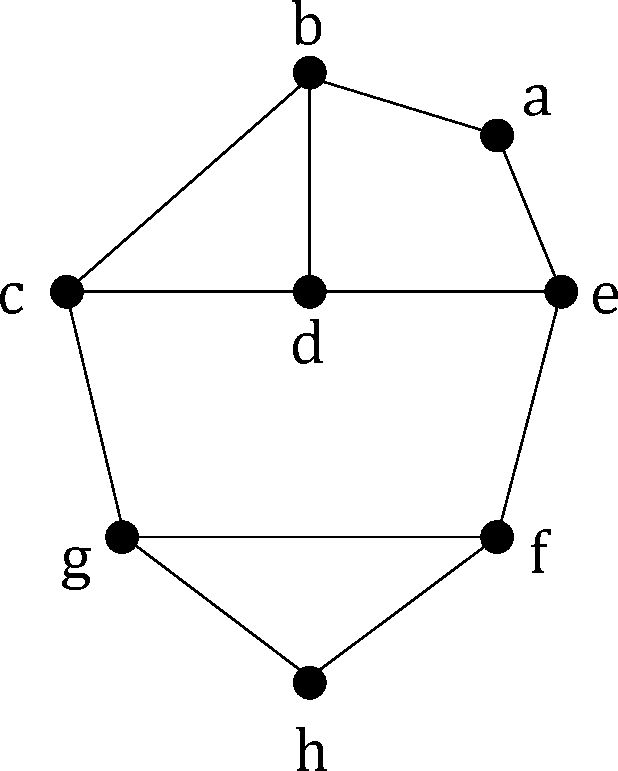
\includegraphics[width = 0.8\textwidth]{2_7_G.pdf}
%                         \caption{$G$}
%                         \label{fig:2_7_G}
%                     \end{subfigure}
%                     % \hfill
%                     \begin{subfigure}[b]{0.4\textwidth}
%                         \centering
%                         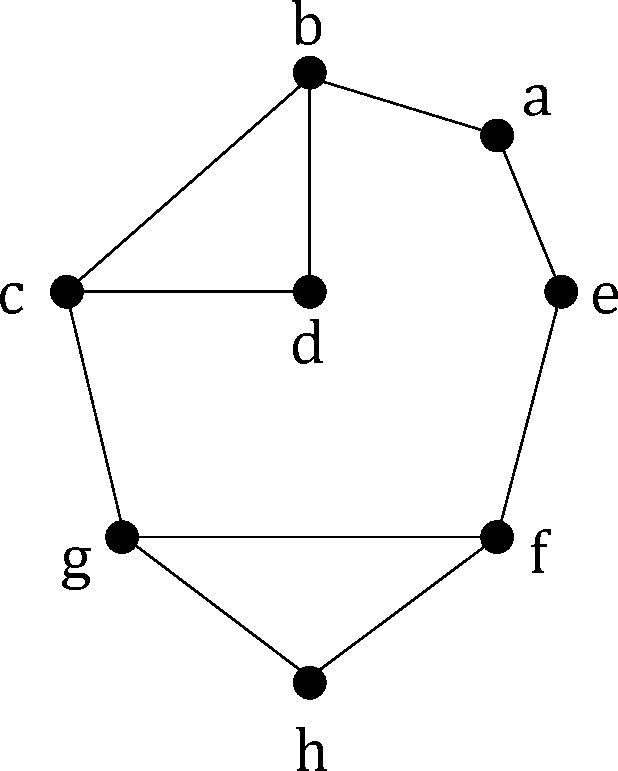
\includegraphics[width = 0.8\textwidth]{2_7_G-d_e.pdf}
%                         \caption{$G-(d,e)$}
%                         \label{fig:2_7_G-d_e}
%                     \end{subfigure}
%                     % \hfill
%                     \begin{subfigure}[b]{0.4\textwidth}
%                         \centering
%                         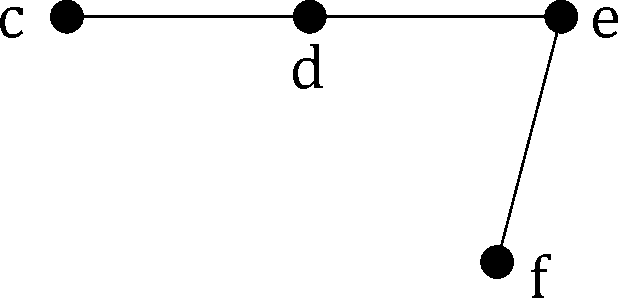
\includegraphics[width = 0.8\textwidth]{2_7_c_d_e_f.pdf}
%                         \caption{$G$ induced by $\{c, d, e, f\}$}
%                         \label{fig:2_7_c_d_e_f}
%                     \end{subfigure}
%                     % \hfill
%                     \begin{subfigure}[b]{0.4\textwidth}
%                         \centering
%                         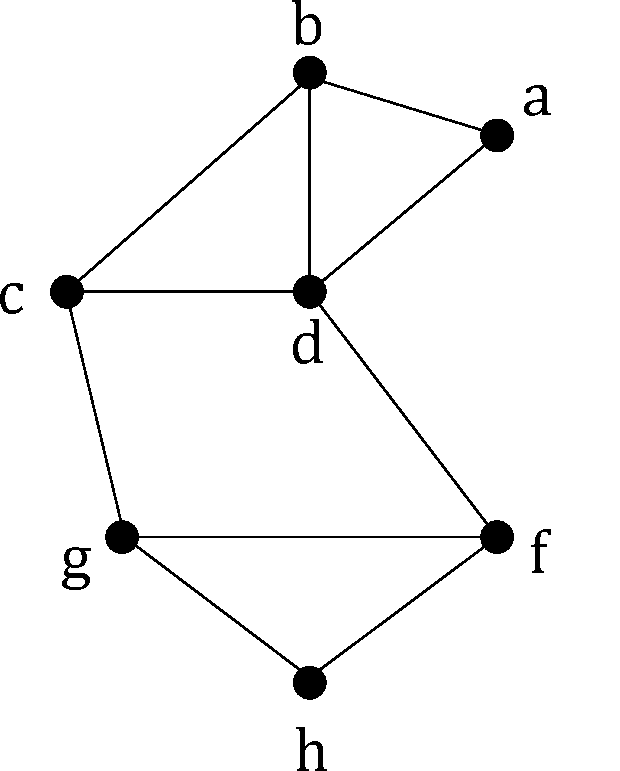
\includegraphics[width = 0.8\textwidth]{2_7_G-d_e_contr.pdf}
%                         \caption{$(d, e)$ edge contracted from $G$}
%                         \label{fig:2_7_G-d_e_contr}
%                     \end{subfigure}
                    
%                     \caption{Graph drawings}
%                     \label{fig:2_7}
%                 \end{figure}
%             }
%         \end{description}
%       }
%       \item {
%         % Show that two graphs are isomorphic if and only if their complements are isomorphic.
        
%         \begin{description}[leftmargin=0em]
%           \item[Answer:] {
%                 Let graph $G$ be isomorphic to $H$, and let $\overline G$, $\overline H$ denote their complements. \\
%                 Since $G$ is isomorphic to $H$, then there exists a bijection $f: V(G) \to V(H)$, such that $(u, v) \in E(G)$ if and only if $(f(u), f(v)) \in E(H)$. \\
%                 Equivalently, there exists a bijection $f: V(G) \to V(H)$, such that $(u, v) \notin E(G)$ if and only if $(f(u), f(v)) \notin E(H)$. \\
%                 Since the vertex set of $G$ and $\overline G$ are the same, therefore $f$ is a bijection from $V(\overline G)$ to $V(\overline H)$. Then suppose $(u, v) \notin E(G)$, by definition of a complement, $(u, v) \in E(\overline G)$. Likewise, if $(f(u), f(v)) \notin E(H)$, then $(f(u), f(v)) \in E(\overline H)$. \\
%                 Hence $\overline G$ and $\overline H$ are isomorphic. \cite{2451171}
%             }
%         \end{description}
%       }
%     \end{enumerate}
